\documentclass{nle}

\usepackage{graphicx,epsfig,subfigure}
\usepackage{multicol}
%%% Load packages
%\usepackage{amsthm}
\usepackage{amsmath}
\usepackage{color}
%\RequirePackage{natbib}
%\RequirePackage{hyperref}
\usepackage[utf8]{inputenc} %unicode support
\usepackage[round]{natbib} 
%\usepackage[applemac]{inputenc} %applemac support if unicode package fails
%\usepackage[latin1]{inputenc} %UNIX support if unicode package fails
\def\newblock{}


%%%%%%%%%%%%%%%%%%%%%%%%%%%%%%%%%%%%%%%%%%%%%%%%%
%%                                             %%
%%  If you wish to display your graphics for   %%
%%  your own use using includegraphic or       %%
%%  includegraphics, then comment out the      %%
%%  following two lines of code.               %%
%%  NB: These line *must* be included when     %%
%%  submitting to BMC.                         %%
%%  All figure files must be submitted as      %%
%%  separate graphics through the BMC          %%
%%  submission process, not included in the    %%
%%  submitted article.                         %%
%%                                             %%
%%%%%%%%%%%%%%%%%%%%%%%%%%%%%%%%%%%%%%%%%%%%%%%%%
\usepackage{setspace}


%%\title{Deep-neural network approaches to speech recognition in heterogeneous groups of speakers including children}
\title[DNN approaches for ASR with heterogeneous groups of speakers]{Deep-neural network approaches for speech recognition with heterogeneous groups of speakers including children}




\author[Romain Serizel and Diego Giuliani]{R\ls O\ls M\ls A\ls I\ls N\ns S\ls E\ls R\ls I\ls Z\ls E\ls L\\
Institut Mines-Télécom/Télécom ParisTech, CNRS-LTCI\\
37, rue Dareau, Paris, France 75014\\
and \\
HLT research unit, Fondazione Bruno Kessler (FBK)\\
Via Sommarive 18, Trento, Italy 38121
\and
and\ns D\ls I\ls E\ls G\ls O\ns G\ls I\ls U\ls L\ls I\ls A\ls N\ls I\\
HLT research unit, Fondazione Bruno Kessler (FBK)\\
Via Sommarive 18, Trento, Italy 38121}





\begin{document}
\label{firstpage}
\maketitle
%\doublespacing
\begin{abstract} % abstract
This paper introduces deep neural network  (DNN) -  hidden  Markov model (HMM) based methods to tackle speech recognition in heterogeneous groups of speakers including children. We target three speaker groups consisting of children, adult males and adult females. Two different kinds of approaches are introduced here: approaches based on DNN adaptation and approaches relying on vocal-tract length normalisation (VTLN).

First, the recent approach that consists
in adapting a general DNN to domain/language specific data is extended
to target  age/gender groups  in the context  of DNN-HMM. Then, VTLN is investigated by training a DNN-HMM system by using either mel frequency cepstral coefficients (MFCC) normalised with standard VTLN or MFCC derived acoustic features combined with the posterior probabilities of the VTLN warping factors. In this later, novel, approach the posterior probabilities of the warping factors are obtained with a separate DNN and the decoding can be operated in a single pass when standard VTLN approach requires two decoding passes. Finally, the different approaches presented here are combined to take advantage of their complementarity. System combination approaches are shown to improve the baseline phone error rate performance by 30\% to 35\% relative and the baseline word error rate performance by about 10\% relative. For clarity sake, the scope of this paper is voluntarily limited to approaches based only on acoustic modelling and features transform based on VTLN.
\end{abstract}

\section{Introduction}
Speaker-related  acoustic variability is a major  source of
errors in automatic  speech recognition.  In this  paper we cope
with  age  group differences,  by  considering  the  relevant case  of
children versus adults, as well as with male/female differences. 
Here DNN is used to deal with the acoustic variability induced by  age and gender differences.

Developmental  changes in  speech  production introduce  age-dependent
spectral and  temporal variabilities  in speech produced  by children.
Studies    on    morphology    and    development   of    the    vocal
tract~\citep*{FitGie99} reveal that during  childhood there is a steady
gradual  lengthening of the  vocal tract  as the  child grows  while a
concomitant        decrease        in       formant        frequencies
occurs~\citep*{HubStaCurAshJoh99,LeePotNar99}.    In   particular,  for
females there is an essential gradual continuous growth of vocal tract
through puberty  into adulthood, while for males  during puberty there
is a disproportionate growth of  the vocal tract, which lowers formant
frequencies, together with an enlargement of the glottis, which lowers
the pitch. After  age 15, males show a  substantial longer vocal tract
and lower formant frequencies than females.  As consequence, voices of
children tend to be more similar  to the voices of women than to those
of men.

When an ASR system trained  on adults' speech is employed to recognise
children's speech,  performance decreases drastically,  especially for
younger children~\citep*{WilJac96,ClaDolBosCom98,DasNixPic98,LiRus01,GiuGer03,PotNar03,GerGiuBru07,Gerosa2009}.
A number of attempts have been reported in the literature to contrast this
effect.   Most of  them  try to  compensate  for spectral  differences
caused by differences  in vocal tract length and  shape by warping the
frequency axis  of the speech power  spectrum of each  test speaker or
transforming                      acoustic                      models
~\citep{ClaDolBosCom98,DasNixPic98,PotNar03}.     However,    to
ensure  good  recognition  performance, age-specific  acoustic  models trained on speech collected  from children of the target age, or
group        of         ages,        is        usually        employed
~(\citealp{WilJac96}; \citealp*{HagPelCol03,NisLeeSarShi04}; \citealp{GerGiuBru07}). Typically
much  less   training  data  are  available  for   children  than  for
adults. The use of adults' speech for reinforcing the training data in
the  case of  a  lack of  children's  speech was  investigated in  the
past~(\citealp{WilJac96}; \citealp*{SteSteHacNotNie03}).  However,  in order to achieve
a recognition performance improvement  when training with a mixture of
children's  and  adults'  speech,  speaker normalisation  and  speaker
adaptive      training      techniques are      usually  needed~\citep*{GerGiuBru09}.

% On the other hand, for adults, variations in voice characteristics due
% to  speaker  age  are much  less  evident  than  for children.   As  a
% consequence,  for adults, recognition  performance is  less correlated
% with age, at least for ASR applications addressing speakers in the age
% range 18-70~\cite{WilJac96}.  In this  study, children and adults are
% considered  as two  homogeneous groups  with respect  to  variations in
% voice characteristics due to speaker age.

How to  cope with acoustic  variability induced by  gender differences
has been studied  for adult speakers in a  number of papers.  Assuming
that there is enough training  data, one  approach  consists in  the use  of
gender-dependent  models   that  are  either  directly   used  in  the
recognition process itself~\citep*{YocMor92,WooOdeValYou94} or used as a
better  seed for  speaker  adaptation~\citep*{LeeGau93}.  Alternatively,
when training  on speakers of both genders,  speaker normalisation and
adaptation  techniques  are  commonly  employed to  contrast  acoustic
inter-speaker variability \citep*{LeeRos96,Gal98}.

Since the  surfacing of  efficient pre-training algorithms  during the
past years~\citep*{hinton06,bengio07,erhan10,seide11}, DNN has proven to
be an  effective alternative to  Gaussian  mixture modelisation
(GMM) in  HMM-GMM based ASR~\citep*{bourlard94,hinton12} and  really good
performance    has     been    obtained    with     hybrid    DNN-HMM
systems~\citep*{dahl12,mohamed12}.

Capitalising  on their good  classification and  generalisation capabilities
the  DNN have  been used  widely in  multi-domain  and multi-languages
tasks~\citep*{sivadas04,stolcke06}.  The  main idea is  usually to first
exploit  a task  independent  (multi-lingual/multi-domain) corpus  and
then to  use a task specific  corpus.  These different  corpora can be
used to design new DNN architectures with application to task specific
ASR~\citep*{pinto09}  or  task  independent ASR~\citep*{bell13}.   Another
approach consists in using the different corpora at different stages of
the DNN  training. The  task independent corpus  is used only  for the
pre-training~\citep*{swietojanski12}      or       for      a  general    first
training~\citep*{vietbac10,thomas13} and the task specific corpus is used
for  the  final  training/adaptation  of the  DNN.   In  under-resourced
scenarios, approaches based on  DNN~\citep*{imseng13} have then shown to
outperform approaches based on  subspace GMM~\citep*{burget13}.

However, to our best knowledge, apart from the very recent work on the
subject in~\citet*{MatChe2014}  DNN is scarcely  used in the  context of
children's  speech recognition.   In~\citet*{Wollmer11}  a bidirectional
long short-term  memory network is  used for keyword detection  but we
have not found any mention of the application of the hybrid DNN-HMM to
children's speech recognition.

Three target groups  of speakers are considered in  this work, that is
children,  adult males  and adult  females.  There  is only  a limited
amount  of  labelled  data  for  such  groups.   We  investigated  two
approaches for ASR in under-resourced conditions with an heterogeneous
population of speakers.

The  first  approach  investigated   in  this  paper  extends  the  idea
introduced in~\citet{YocMor92} to the  DNN context.  The DNN trained on
speech data  from all the three  groups of speakers is  adapted to the
age/gender group specific corpora.  First  it is shown that training a
DNN  only from  a group  specific corpus  is not  effective  when only
limited  labelled  data  is   available.   Then  the  method  proposed
in~\citet{thomas13} is  adapted to the age/gender  specific problem and
used in a DNN-HMM architecture instead of a tandem architecture.

The second approach introduced in this paper relies on VTLN. 
In~\citet{seide11} an  investigation was conducted  by training a
DNN on VTLN normalised acoustic features, it was found that in a large
vocabulary  adults'  speech  recognition  task  limited  gain  can  be
achieved with respect to using un-normalised acoustic features.  It was
argued that, when  a sufficient amount of training  data is available,
DNN   are  already   able  to   learn,  to   some   extent,  internal
representations  that  are  invariant   with  respect  to  sources  of
variability such as  the vocal tract length and  shape.  However, when
only  limited  training  data   is  available  from  a  heterogeneous
population of speakers,  made of children and adults  as in our case,
the   DNN   might   not    be   able   reach   strong   generalisation
capabilities~\citep*{SerGiu2014}.   In such  case,  techniques like  DNN
adaptation~\citep{vietbac10,swietojanski12,thomas13}, speaker
adaptation~\citep*{abdel2013rapid,liao2013speaker} or
VTLN~(\citealp*{EidGis96}; \citealp{LeeRos96}; \citealp*{WegMcaOrlPek96})  can help to  improve the
performance. Here we consider  first the application of a conventional
VTLN technique to normalise MFCC as input features to a DNN-HMM system.

Recent  works have shown  that augmenting  the inputs  of a  DNN with,
e.g.  an  estimate  of  the background  noise~\citep*{export:194344}  or
utterance  i-vector~\citep*{42536},  can   improve  the  robustness  and
speaker independence of  the DNN. We then propose  to augment the MFCC
inputs of the DNN with the posterior probabilities of the VTLN-warping
factors to  improve robustness with respect  to inter-speaker acoustic
variations.

This   paper  extends   previous  work   by  the   authors   on  DNN
adaptation~\citep{SerGiu2014}      and      VTLN     approaches      for
DNN-HMM based ASR~\citep*{SerGiu2014a}.  An approach to  optimise jointly  the DNN
that extracts the posterior probabilities of  the warping factors and the DNN-HMM is
proposed here,  combination of the different  approaches is considered
and the different systems performance  are evaluated not only on phone
recognition but also on word recognition. 

This paper is a proof of concept and the authors voluntarily limited its focus to simple ASR systems. Only  age and gender groups problems and approaches based only on acoustic modeling and VTLN transform are considered here in order to focus on the effects of these particular approaches. Therefore state-of-the-art approaches based on speaker identity models such as I-vectors~(\citealp*{dehak2011front,saon2013speaker}; \citealp{42536}), speaker codes~\citep*{abdel2013fast}, linear input networks and linear output networks~\citep*{li2010comparison} are beyond the scope of this paper. At this initial stage, the authors decided to focus on approaches based only on acoustic modelling therefore excluding approaches requiring an entire decoding stream (or at least a language model), such as approaches based on confusion networks~\citep*{mangu2000finding}.

The    rest    of    the    paper    is    organised    as    follows,
Section~\ref{section:DNN}   briefly   introduces   DNN  for   acoustic
modelling   in   ASR  and   present   the   approach   based  on   DNN
adaptation.    Approaches   based   on    VTLN   are    presented   in
Section~\ref{section:VTLN}.  The experimental  set-up  is described  in
Section~\ref{section:expS}  and experiments  results are  presented in
Section~\ref{section:expR}.  Finally,  conclusions  of the  paper  are
drawn in Section~\ref{section:concl}.

\section{DNN adaptation}\label{section:DNN}
A DNN is a feed-forward neural network where the neurons are arranged in fully connected layers. The input layer processes the feature vectors (augmented with context) and the output layer provides (in the case of ASR) the posterior probability of the (sub)phonetic units. The layers between the input layer and the output layer are called hidden layers. DNN are called deep because they are composed of many layers. Even though shallow neural network architectures (i.e., with few hidden layers) are supposed to be able to model any function they may require a huge of parameters to do so. The organisation of the neurons in a deep architecture allows to use parameters more efficiently and to model the same function as a shallow architectures with less parameters~\citep*{bengio2013representation}. Deep architectures also allow to extract high level features that are more invariant (and therefore more robust) than low level features~\citep{hinton12}. They also allow to close the 
semantic gap between the features and the (sub)phonetic units. 

The DNN used in this papers have sigmoid activation functions in the hidden layers:
\begin{align}
h & = \textbf{w}.\textbf{y} + b\nonumber\\
  \sigma(h) & = \frac{1}{1+ e^{-h} }\nonumber
\end{align}
with $\textbf{y}$ the vector of input to the layer, $\textbf{w}$ the weights of the layer and $b$ the bias of the layer.

The target of the DNN presented here is to estimate posteriors probabilities. Therefore, it is chosen to use softmax activation in the output layer, as the the output then sum up to one:
\begin{equation}
 softmax(\textbf{h}_j)=\frac{e^{h_j}}{\sum\limits_i e^{h_i}}\nonumber
\end{equation}

The posterior probabilities are then normalised by the prior probabilities of the observation to obtain the state emission likelihood used by the HMM. Following Bayes rule:
\begin{equation}
 p(X|S)\propto \frac{p(S|X)}{p(S)} \nonumber
\end{equation}

Where $X$ is the observation and $S$ the HMM state.

\subsection{Pre-training/training procedure}
Training a DNN is a difficult tasks mainly because the optimisation criterion involved is non convex. Training a randomly initialised DNN with back-propagation would converge to one of the many local minima involved in the optimisation problem sometimes leading to poor performance~\citep{erhan10}. In recent works this limitation has been partly overcome by training on a huge amount of data (1700 hours in~\citet{42536}). However, this solution does not apply when tackling ASR for under-resourced groups of population where the amount of training data is limited by definition. In such cases, pre-training is a mandatory step to efficiently train a DNN. The aim of pre-training is to initialise the DNN weights to a better starting point than randomly initialised DNN and avoid the back-propagation training to be stuck in a poor local minima. Here generative training based on Restricted Boltzmann Machines (RBM)~\citep{hinton06,erhan10} is chosen. Once the DNN weights have been initialised with stacked RBM, the DNN is trained to convergence with back-propagation. More details about training and network parameters are presented in Sections~\ref{sssection:exp:DNN} and~\ref{sssection:exp:DNNW}.

\subsection{Age/gender independent training} 
The general training procedure described above can be applied, by using
all training data available, in an attempt to  achieve   a  system  with   strong  generalisation  capabilities.
Estimating the DNN  parameters on speech from all  groups of speakers,
that is  children, adult  males and adult  females, may however, have
some limitation due to the  inhomogeneity of the speech data that may
negatively   impact  on  the   classification  accuracy   compared  to
group-specific DNN.

\subsection{Age/gender adaptation}
ASR  systems  provide their  best  recognition  performances when  the
operating  (or testing)  conditions match   the training
conditions.  To be effective, the general training procedure described
above requires that a sufficient  amount of labelled data is available.
Therefore,  when considering  training  for under-resourced  population groups
(such  as   children  or   males/females  in  particular   domains  of
applications) it  might be more  effective to train  first a DNN  on all
data available and then to adapt this DNN to a specific group of speakers. 
A similar approach has been proposed in~\citet{thomas13} for  the  case of  multilingual training.
Here the language  does not change and the targets of the DNN remain
the same when going from age/gender independent training to group
  specific adaptation.  The DNN trained on speech data from all groups
  of  speakers can  then be  used  directly as  initialisation to  the
  adaptation  procedure where  the DNN  is trained  to convergence
  with back-propagation only on group specific speech corpora.
  
This adaptation approach, however, suffers from a lack of flexibility: 
a new DNN would have to be adapted to each new group of speakers.
  
\section{VTLN approaches}\label{section:VTLN}
In this section, we propose to define a more general framework inspired by VTLN approaches to ASR to tackle the problem of inter-speaker acoustic variability due to
vocal tract  length (and shape)  variations among speakers. Two different approaches are considered here. The  first  one  is  based  on  the
conventional   VTLN  approach~\citep{EidGis96,LeeRos96,WegMcaOrlPek96}.
The resulting VTLN  normalised acoustic features are used  as input to
the  DNN both during  training and  testing~\citep{seide11}.  The
second approach, proposed in this  paper, has two main features: a) by
using a dedicated DNN, for each speech frame the posterior probability
of each warping  factor is estimated and b) for  each speech frame the
vector  of the  estimated  warping factor  posterior probabilities  is
appended to  the un-normalised acoustic features  vector, extended with
context, to form an augmented  acoustic features vector for the DNN-HMM
system.

\subsection{VTLN normalised features as input to the DNN}
In   the   conventional   frequency   warping  approach   to   speaker
normalisation~\citep{EidGis96,LeeRos96,WegMcaOrlPek96},  typical issues
are  the estimation  of a  proper  frequency scaling  factor for  each
speaker, or utterance, and the implementation of the frequency scaling
during  speech  analysis.  A  well  known  method  for estimating  the
scaling  factor is  based on  a  grid search  over a  discrete set  of
possible scaling  factors by maximizing the likelihood  of warped data
given  a  current set  of  HMM-based acoustic  models~\citep{LeeRos96}.
Frequency scaling  is performed by  warping the power  spectrum during
signal  analysis  or, for  filter-bank  based  acoustic front-end,  by
changing the  spacing and width  of the filters while  maintaining the
spectrum  unchanged~\citep{LeeRos96}.   In  this  work we  adopted  the
latter approach considering a discrete set of VTLN factors. Details on the VTLN implementation  are provided in
Section~\ref{sssection:exp:VTLN}.

Similarly to the method proposed in~\citet{seide11}, the VTLN normalised
acoustic features are used to form the input to the DNN-HMM system both
during training and testing.

\subsection{Posterior probabilities of VTLN warping factors as input to DNN}
In this  approach we propose  to augment the acoustic  features vector
with the posterior probabilities of  the VTLN warping factors to train
a warping-factor  aware DNN.   Similar approaches have  recently been
shown  to  improve the  robustness  to noise and  speaker  independence of  the
DNN~\citep{export:194344,42536}.

The VTLN procedure is first applied to generate a warping factor for
each  utterance in the  training set. Each acoustic feature vector in the utterance is labelled with the utterance warping factor. Then, training acoustic feature vectors and corresponding warping factors are used to train a DNN classifier. Each class of the DNN correspond to one of the discrete VTLN factors and the dimension of the DNN output corresponds to the number of discrete VTLN factors. The DNN learns to infer the VTLN warping factor from the acoustic feature vector (Figure~\ref{fig1}) or more precisely the posterior probability of each VTLN factors knowing the input acoustic feature vector. This DNN will be referred to as DNN-warp.
\begin{figure}
       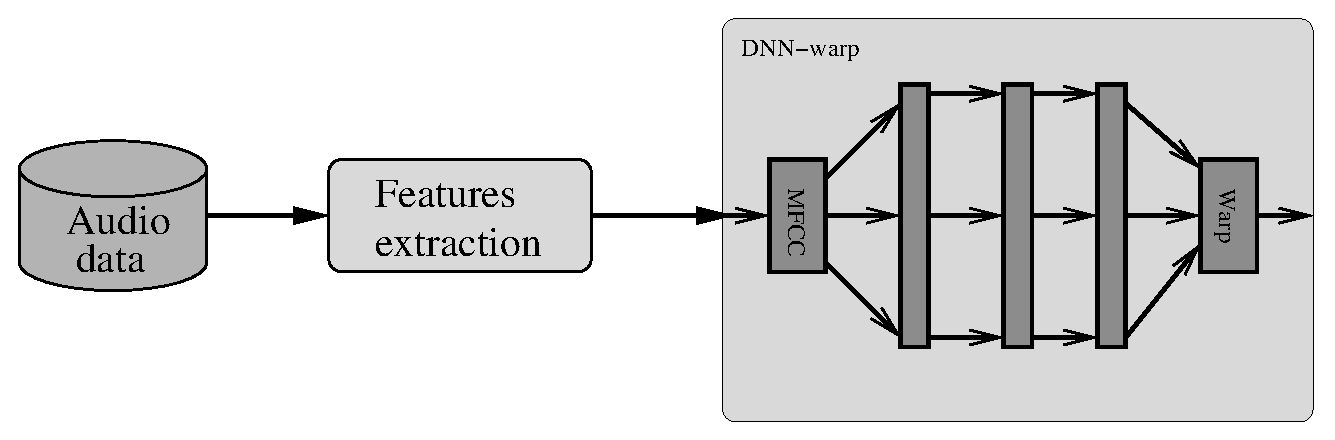
\includegraphics[width=\textwidth]{fig1}
        \caption{Training of the DNN-warp.} 
   	\label{fig1}
\end{figure}

% HERE: the generation the augmented feature vector is described  twice
%
% The feature vector augmented with context is
% combined  with these  posterior  probabilities and  the new  augmented
% feature vector is  normalised and used to train  a DNN acoustic model.
%
% Answer: I removed the part above but kept the part below to explain how the system runs at decoding time

At  decoding time,  the DNN-warp  is  used to  produced the  posterior probabilities of  the warping factors which are  then concatenated with the acoustic  feature vector  (with context).  The  augmented features vector is used as input to the warping-factor aware DNN acoustic model to produce  posterior probabilities of the  triphone tied-states. This procedure  has the  advantage  to reduce  considerably the  complexity during decoding compared to standard VTLN~\cite{LeeRos96}.


During training  and testing  of the DNN-HMM  system, for  each speech
frame the  warping factors posterior probabilities are  estimated with
the DNN-warp. These estimated  posterior probabilities are appended to
the un-normalised acoustic feature vectors, extended  with context, to
form an augmented acoustic feature vectors. Mean and variance normalisation is then applied to the extended features vector
which is used as input to the DNN-HMM (Figure~\ref{fig2}).
 \begin{figure}
       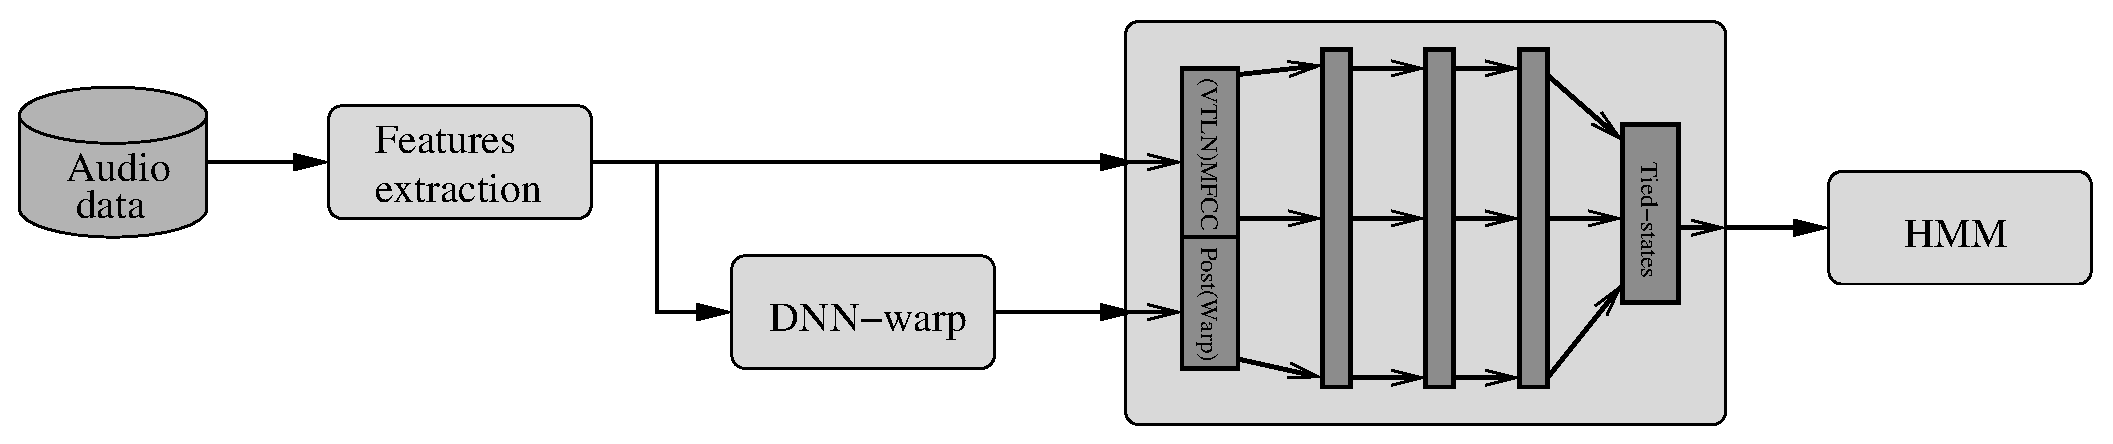
\includegraphics[width=\textwidth]{fig2}
         \caption{Training of the warping factor aware DNN-HMM.} 
    	\label{fig2}
 \end{figure}
 
This approach has the  advantage to reduce considerably the complexity
during decoding compared to the approach making use of VTLN normalised
acoustic features that requires two decoding passes~(\citealp{LeeRos96}; \citealp*{WelKanNey99}). It also allows for flexible estimation of the warping factors: they could either be updated on a frame to frame basis or averaged at utterance level (see also Section~\ref{section:expR}).

\subsection{Joint optimisation}
The ultimate goal here is not to estimate the VTLN warping factors but to perform robust speech recognition on heterogeneous corpora. To this end, the DNN-warp and the DNN-HMM can be optimised jointly (Figure~\ref{fig3}). The procedure is the following one: 1) first the DNN-warp is trained alone (Figure~\ref{fig1}), 2) the posteriors of the warping factors on the training set are obtained with the DNN-warp, 3) these posteriors of the warping factors are used as input to the DNN-HMM together with the acoustic features to produce an extended feature vector, 4) the DNN-HMM is trained (Figure~\ref{fig2}), 5)  the DNN-warp and the DNN-HMM are concatenated to obtained a deeper network that is fine-tuned with back-propagation on the training set (Figure~\ref{fig3}). Details about joint optimisation are presented in Section~\ref{sssection:exp:joint}

  \begin{figure}
       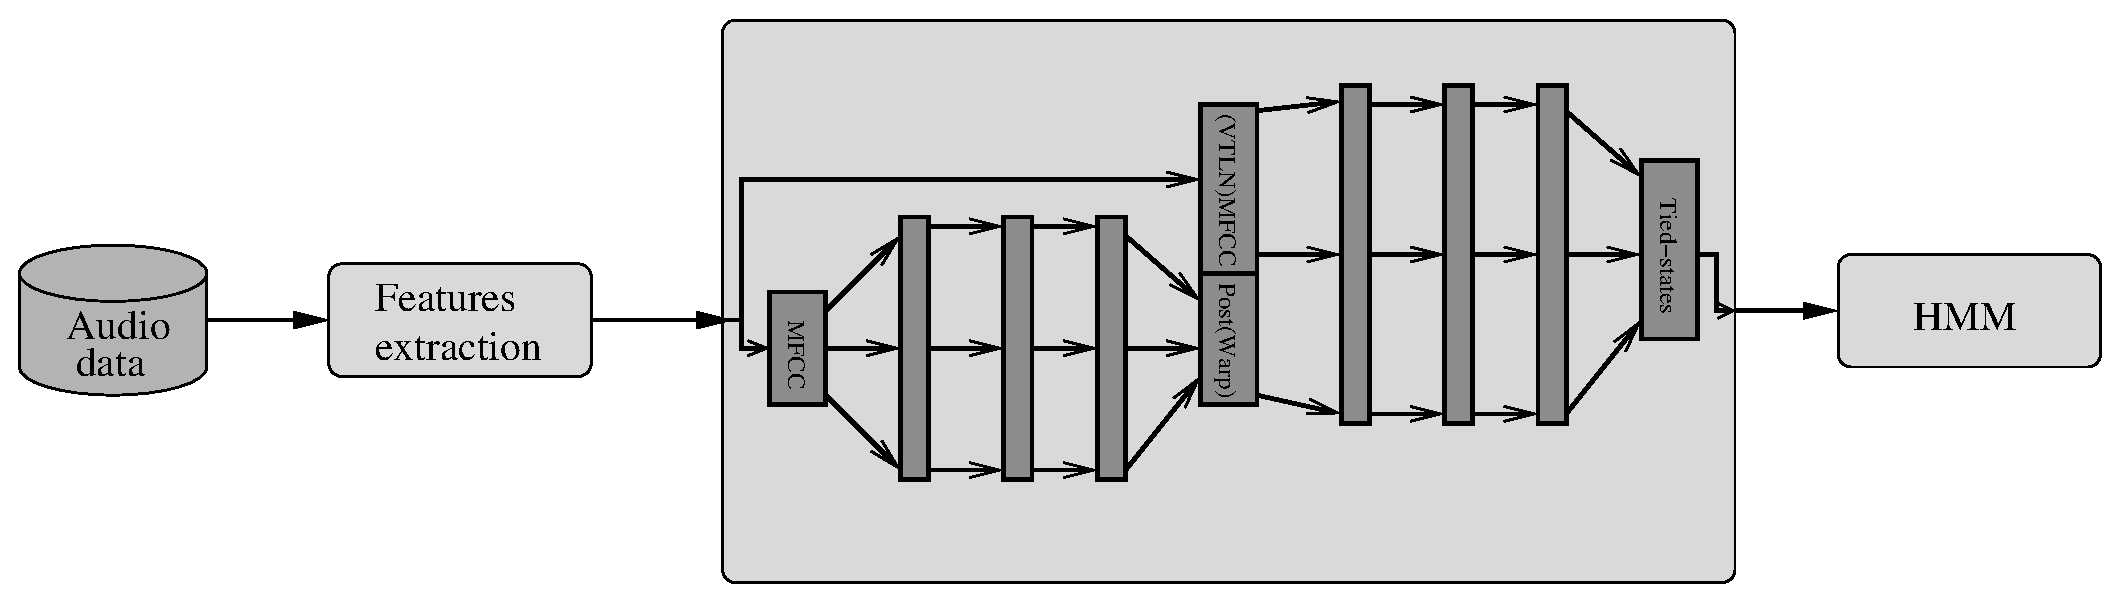
\includegraphics[width=\textwidth]{fig3}
          \caption{Joint optimisation of the DNN-warp and the DNN-HMM.} 
     	\label{fig3}
  \end{figure}

\section{Experimental set-up}\label{section:expS}
\subsection{Speech corpora}

For  this study  we  relied  on three  Italian  speech corpora:  the
ChildIt corpus  consisting of children speech,  the APASCI corpus and the IBN corpus consisting of  
adults'  speech.    All  corpora  were  used  for
evaluation purposes, while the ChildIt and the APASCI provided similar
amount of training data for children and adults, respectively, IBN corpus contains  approximately 5 times as much training data as ChildIt or APASCI (Table~\ref{tab0}).

\begin{table}

  \begin{minipage}{\textwidth} 
\begin{tabular}{lrrrrr}
\hline \hline
         &\multicolumn{5}{ c} {Speech Corpus}\\ 
         &ChildIt&APASCI(f)&APASCI(m)&IBN(f)&IBN(m)\\ \hline
Train&7h:15m &  2h:40m&  2h:40m&23h:00m&25h:00m\\\noalign{\vspace {.5cm}}
Test&  2h:20m &  0h:20m&0h:20m& 1h:00m& 1h:00m\\
\hline\hline
\end{tabular}
\end{minipage}
\caption{Data repartition in the speech corpora. (f) and (m) denote speech from female and male speakers, respectively. \label{tab0}}

\end{table}


\subsubsection{ChildIt}

The  ChildIt corpus~\citep{GiuGer03,GerGiuBru07}  consists  of Italian
read sentences  collected from  171 children (86  male and  85 female)
aged between 7  and 13, with a mean age of  10 years.  Recordings took
place at school, usually in the computer room or in the library.  Each
child  was asked  to read  a set  of sentences  prepared  according to
her/his  grade.   Figure~\ref{ChildItAge} reports the distribution of children per grade.


\begin{table}
  \begin{minipage}{\textwidth}
\begin{tabular}{cccccccc}
\hline \hline
        & \multicolumn{7}{c} {Grade} \\
        & 2  &  3  & 4   & 5   & 6   & 7    & 8 \\ \hline
 N. Speakers       & 24 &  24 & 23  & 24  & 28  &  26  & 22 \\ \hline\hline
\end{tabular}
\end{minipage}
\caption{Distribution of speakers in the ChildIt corpus per grade. Children in grade 2 are approximatively 7 years old while children in grade 8 are approximatively 13 years old. \label{ChildItAge}}

\end{table}


The overall  duration of audio recordings in  the corpus is
10h:24m. For  all  recordings  in  the  corpus  a
word-level   transcription   is  available.    

The corpus was partitioned into: a training set  consisting of data from 115 speakers
for a  total duration of 7h:15m;  a development set  consisting of data
from  14  speakers,  for a  total  durations  of  0h:49m; a  test  set
consisting of data  from 42 speakers balanced with  respect to age and
gender for a total duration of of 2h:20m.


\subsubsection{APASCI}
The    APASCI   speech    corpus~\citep*{AngBruFalGiuGreOmo94}    is   a
task-independent,    high     quality,    acoustic-phonetic    Italian
corpus. For recordings in the corpus a word-level transcription is available. APASCI was  developed at ITC-irst and consists  of speech data collected from  194 adult  speakers for a  total durations  of 7h:05m.
The corpus  was partitioned  into: a training  set consisting  of data
from 134  speakers for a total  duration of 5h19m;  a development set
consisting of data  from 30 speakers balanced per  gender, for a total
durations of  0h39m; a test set  consisting of data  from 30 speakers
balanced per gender, for a total duration of 0h40m.

\subsubsection{IBN Corpus}
The IBN corpus is composed of speech from several radio and television
Italian news programs~\citep{GerGiuBru09}. It consists of adult speech
only, with word-level transcriptions. The IBN corpus was  partitioned into a training set, consisting
of 52h:00m of speech, and a test set formed by 2h:00m of speech. During the experiments presented here 2h:00m of male speech and 2h:00m of female speech are extracted from the training set to be used as development set during the DNN training. The resulting training set is then partitioned into 25h:00m of male speech and 23h:00m of female speech.

% The  IBN training  set  includes  also  two small  task
% independent   corpora  called   APASCI  and   SPEEDATA.    The  APASCI
% corpus~\cite{AngBruFalGiuGreOmo94}   is   a  task-independent,   high
% quality,   acoustic-phonetic   Italian   database.   Acquisition   was
% performed in  quiet rooms  using a digital  audio tape recorder  and a
% high-quality close-talk microphone.  Audio signals were acquired at 48
% kHz sampling  frequency and  then down-sampled to  16 kHz with  16 bit
% accuracy.  Only a portion of  APASCI corpus, consisting of speech from
% 124 speakers  (for an  overall duration of  5h:38m), was  exploited in
% this work  for speech analysis  purposes and acoustic  model training.
% The   SPEEDATA  corpus~\citep{AckAngBruFedGiuGreNie97}  is   a  corpus
% designed and collected by ITC-irst with criteria very similar to those
% adopted for APASCI and consisting of about 5h:48m of speech.

\subsection{Phone recognition systems}
The approaches proposed in this paper have been first tested on small
corpora (ChildIt + APASCI) for phone recognition to explore as many
set-ups as possible in a limited amount of time.  The
reference phone transcription of an utterance was derived from the
corresponding word transcription by performing Viterbi decoding on a
pronunciation network.  This pronunciation network was built by
concatenation of the phonetic transcriptions of the words in the word
transcription.  In doing this alternative word pronunciations were
taken into account and an optional insertion of the silence model
between words was allowed.

%The reference phone-level transcriptions are obtained with Viterbi forced-alignement performed with our best GMM-HMM system at the moment of the experiments.
\subsubsection{GMM-HMM}\label{sssection:base}

The  acoustic  features are  13  mel  frequency cepstral  coefficients
(MFCC), including the zero order coefficient, computed on 20ms frames
with 10ms overlap.  First, second and third order time derivatives are
computed  after  cepstral  mean  subtraction  performed  utterance  by
utterance.  These  features are arranged into  a 52-dimensional vector
that is  projected into a  39-dimensional feature space by  applying a
linear   transformation  estimated   through   Heteroscedastic  Linear
Discriminant Analysis (HLDA)~\citep*{Kumar1998283}.

Acoustic models  are 3039 tied-state  triphone HMM
based on  a set of  48 phonetic units  derived from the  SAMPA Italian
alphabet.  Each  tied-state  is modelled with  a mixture of  8 Gaussian
densities   having  a  diagonal   covariance  matrix.    In  addition,
``silence''  is  modelled  with  a  Gaussian mixture  model  having  32
Gaussian densities.

\subsubsection{DNN-HMM}\label{sssection:exp:DNN}
The DNN  uses again  13 MFCC, including  the zero  order coefficient,
computed on 20ms  frames with 10ms overlap. The context  spans on a 31
frames  window. For each frequency band, the 31 coefficients context is separately scale with Hamming and projected to a 16 dimensional vector using DCT. The 13 resulting vectors are concatenated to obtain a 208 dimensional feature  vector which is normalised to have zero-mean and unit variance before being used as input to the DNN. The targets of the
DNN are the 3039 tied-states obtained from the GMM-HMM training on the
mixture of adults'  and children's speech (ChildIt +  APASCI). The DNN
has 4  hidden layers, each of  which contains 1500  elements such that
the DNN architecture can be summarised as follows: 208 x 1500 x 1500 x
1500 x 1500 x 3039.

The DNN are trained with the TNet software package~\citep*{vesely10}. The DNN weights are initialised randomly and pre-trained with RBM. The first layer is pre-trained with a Gaussian-Bernouilli RBM trained during 10 iterations with a learning rate of 0.005. The following layers are pre-trained with a Bernouilli-Bernouilli RBM trained during 5 iterations with a learning rate of 0.05. Mini-batch size is 250. For the back propagation training the learning rate is kept to 0.02 as long as the frame accuracy on the cross-validation set progresses by at least 0.5\% between successive epochs. The learning rate is then halved at each epoch until the frame accuracy on the cross-validation set fails to improve by at least 0.1\%. The mini-batch size is 512. In both pre-training and training, a first-order momentum of 0.5 is applied. The values of the hyper-parameters (network topology and learning parameters) are standard values, in the range of the values commonly used for these parameters in the literature.

The DNN can be trained either on all speech data available  (ChildIt + APASCI) or on group specific corpora (ChildIt, adult female speech in APASCI, adult male speech in APASCI).

\subsubsection{Language model}
A simple finite state network having  just one state and a  looped transition for each
phone  unit   was  employed.   In  this   network  uniform  transition
probabilities  are  associated to  looped  transitions.  In  computing
recognition  performance,  in terms  of  PER,  no
distinction  was made  between  single consonants  and their  geminate
counterparts.  In this way, the  set of phonetic labels was reduced
from 48 to 28 phone labels.  


% Recognition  results  were  always  generated  in  a  single  decoding pass.

\subsection{Word recognition systems}
The approaches that performed best in phone recognition on the small corpora are validated in word recognition on a more realistic set-up (ChildIt+ IBN) including a corpus of adult speech (IBN) that is larger than the corpus of children speech (ChildIt).
\subsubsection{GMM-HMM}\label{sssection:baseW}

The GMM-HMM are similar to those used for phone recognition except that they use more Gaussian densities to benefit from the extensive training data. Acoustic models  are 5021 tied-state  triphone HMM
based on  a set of  48 phonetic units  derived from the  SAMPA Italian
alphabet. Each tied-state is modelled with  a mixture of  32 Gaussian
densities   having  a  diagonal   covariance  matrix. In  addition,
``silence''  is  modelled  with  a  Gaussian mixture  model  having  32
Gaussian densities.


\subsubsection{DNN-HMM}\label{sssection:exp:DNNW}
The DNN  are similar to those  used for phone  recognition except that
they are  trained on a different  set of targets. The  targets of the
DNN are the 5021 tied-states obtained from the word recognition GMM-HMM training on the
mixture of adults' and children's  speech (ChildIt + IBN). The DNN has
4 hidden  layers, each of which  contains 1500 elements  such that the
DNN architecture  can be summarised  as follows: 208  x 1500 x  1500 x
1500 x 1500 x 5021.

\subsubsection{Language model}
For word  recognition, a  5-gram language model  was trained  on texts
from the Italian  news domain consisting in about  1.6G words. Part of
the textual  data, consisting in  about 1.0G words, were  acquired via
web crawling of news  domains.  The recognition dictionary consists of
the most frequent 250K words.

\subsection{Age/gender adapted DNN for DNN-HMM}
One option is to adapt an already trained general DNN  to group specific corpora. The data architecture is the same as described above. The initial DNN weights are the weights obtained with a pre-training/training procedure applied on all training data available  (ChildIt+APASCI, respectively ChildIt + IBN). The DNN is then trained with back propagation on a group specific corpora (ChildIt, adult female speech in APASCI and adult male speech in APASCI, respectively IBN). The training parameters are the same as during the general training (\ref{sssection:exp:DNN} and \ref{sssection:exp:DNNW}, respectively) and the learning rate follows the same rule as above. The mini-batch size is 512 and a first-order momentum of 0.5 is applied.

\subsection{VTLN}\label{sssection:exp:VTLN}
In  this  work  we are considering  a  set   of  25  warping   factors  evenly
distributed, with step 0.02, in the range 0.76-1.24. During both training and testing
a grid search over the 25 warping factors was performed.  The acoustic
models   for   scaling   factor    selection,   carried   out   on   an
utterance-by-utterance  basis, were speaker-independent  triphone HMM
with  1 Gaussian  per state  and  trained on  un-warped children's  and
adults' speech~\citep{WelKanNey99,GerGiuBru07}.

The DNN-warp inputs are the MFCC with a 61 frames context window, DCT
projected to a 208 dimensional features vector the procedure is similar as in \ref{sssection:exp:DNN}). The targets are the 25
warping factors. The  DNN has 4 hidden layers,  each of which contains
500  elements such  that the  DNN  architecture can  be summarised  as
follows: 208 x 500  x 500 x 500 x 500 x  25. The training procedure is
the same as for the DNN  acoustic model in the DNN-HMM.  

The posterior
probabilities  obtained with  the  DNN-warp are concatenated with  the
208-dimensional DCT  projected acoustic  features vector to produce a
233-dimensional features  vector that is mean-normalised  before being used
as input to  the DNN. The new DNN acoustic model  has 4 hidden layers,
each of  which contains 1500  elements such that the  DNN architecture
can then be summarized  as follows: 233 x 1500 x 1500  x 1500 x 1500 x
3039 for phone recognition (233 x 1500 x 1500  x 1500 x 1500 x 5021 for word recognition).

\subsection{Joint optimisation}\label{sssection:exp:joint}
The DNN-warp and DNN-HMM can be fine-tuned jointly with back-propagation. In such case, the starting learning rate is set to 0.0002 in the first 4 hidden layers (corresponding to the DNN-warp) and to 0.0001 in the last 4 hidden layers (corresponding to the DNN-HMM). The learning rate is chosen empirically as the highest value for which both training accuracy and cross-validation accuracy improve. Setting a different learning rate in the first 4 hidden layers and the last 4 hidden layers is done in a attempt to overcome the vanishing gradient effect in the 8 layers DNN obtained from the concatenation of the DNN-warp and the DNN-HMM. The learning rates are then adapted following the same schedule as described above. The joint optimisation is done with a modified version of the TNet software package~\citep{vesely10}.
\section{Experimental Results}\label{section:expR}
Two sets of experiments are presented here. First the systems are tested extensively in terms of PER on small corpora (ChildIt + APASCI), then the best performing systems are tested in terms of WER performance on a more realistic set-up including a larger adult speech corpus (IBN).
\subsection{Phone recognition}

The experiments presented here are designed to verify the validity of the following statements:

\begin{itemize}
 \item The age/gender group specific training of the DNN does not necessarily lead to improved performance, specially when a small amount of data is available
 \item The age/gender group adaptation of a general DNN can help to design group specific systems, even when only a small amount of data is available
 \item VTLN can be beneficial to the DNN-HMM framework when targeting 
a heterogeneous speaker population with limited amount of training data
 \item Developing an "all-DNN" approach to VTLN for DNN-HMM framework, when targeting a heterogeneous speaker population, offers a credible alternative to the use of VTLN normalised acoustic features or to the use of age/gender group specific DNN
 \item Optimising the DNN-warp and the DNN-HMM jointly can help to improve the performance in certain cases
 \item The different approaches introduced in this paper can be complementary.

\end{itemize}
During the experiments the language model weight is tuned on the development set and used to decode the test set.  Results were obtained with a phone loop language model and the PER was  computed based on 28 phone labels. Variations  in recognition performance were  validated using the
matched-pair  sentence test~\citep*{GilCox89}  to ascertain  whether the
observed results  were inconsistent with the null  hypothesis that the
output  of  two  systems  were  statistically  identical.   Considered
significance levels were $.05$, $.01$ and $.001$.

\subsubsection{Age/gender specific  training for DNN-HMM}
In  this  experiment,  DNN  are  trained  on  group  specific  corpora
(children's speech in ChildIt, adult female speech in APASCI and adult
male speech in  APASCI) and performance are compared  with the DNN-HMM
baseline introduced above where the  DNN is trained on speech from all
speaker groups. Recognition  results are reported in Table~\ref{tab1},
which includes results  achieved with the DNN-HMM baseline  in the row
{\em Baseline}. In ChildIt there is about 7h of training data which is
apparently sufficient to train an  effective DNN and we can observe an
improvement of 22\% PER  relative compared to the baseline performance
(from 15.56\% to 12.76\% with $p <.001$). However, in adult data there
is only about  2h:40m of data for each gender.  This is apparently not
sufficient to train a DNN. In  fact, the DNN-HMM system based on a DNN
that  is trained  on gender  specific data  consistently  degrades the
PER. The degradation compared to  the baseline performance is 14\% PER
relative on female speakers in APASCI (from 10.91\% to 12.75\% with $p
<.001$) and 12\% PER relative  on male speakers in APASCI (from 8.62\%
to 9.83\% with $p <.001$).

\begin{table}
\begin{minipage}{\textwidth}
\begin{tabular}{lrrr}
\hline\hline
      &\multicolumn{3}{ c }{Evaluation Set}\\ 
 Training Set &ChildIt&APASCI(f)&APASCI(m)\\\hline 
Baseline&  15\hpt56\% &  \textbf{10\hpt91\%}& \textbf{8\hpt62\%}\\\noalign{\vspace {.5cm}}
ChildIt& \textbf{12\hpt76\%} &  29\hpt59\%&  46\hpt16\%\\\noalign{\vspace {.5cm}}
APASCI(f)& 34\hpt23\% &  12\hpt75\%& 31\hpt21\%\\\noalign{\vspace {.5cm}}
APASCI(m)&  56\hpt11\% & 30\hpt81\%&  9\hpt83\%\\\noalign{\vspace {.5cm}}
\hline\hline 
\end{tabular}
\end{minipage}
\caption{Phone error rate achieved with the DNN-HMM trained age/gender groups specific data.\label{tab1}}
\end{table}

\subsubsection{Age/gender adapted DNN-HMM}
In this  experiment the DNN trained  on all available corpora is
adapted to  each group specific corpus and  recognition performance is
compared with that obtained by  the DNN-HMM baseline (where the DNN is
trained on  all available corpora).   PER performance is  presented in
Table~\ref{tab2}  which  also  reports  the results  achieved  by  the
DNN-HMM  baseline  (in  row  {\em  Baseline}).   The group  adapted
DNN-HMM  consistently improve the  PER compared to  the DNN-HMM
baseline.  On children's  speech the PER improvement compared to the baseline is  25\% PER relative (from 15.56\% to 12.43\% with $p
<.001$). On adult female speakers in APASCI the age/gender adaptation improves the baseline performance by is 13\% PER relative (from  10.91\% to 9.65\% with $p <.001$). On adult male speakers the age/gender adaptation improves the baseline performance by 13\% (from 8.62\%  to  7.61\% with $p<.05$).

\begin{table}
\begin{minipage}{\textwidth}
\begin{tabular}{lrrrrrrr}
\hline\hline
     &\multicolumn{4}{ c }{Evaluation Set}\\ 
Adaptation Set &ChildIt&APASCI(f)&APASCI(m)&ChildIt + APASCI\\\hline 
Baseline& 15\hpt56\% &  10\hpt91\%& 8\hpt62\%&14\hpt32\%\\\noalign{\vspace {.5cm}}
ChildIt& \textbf{ 12\hpt43\%} &  16\hpt93\%&  24\hpt96\%&N/A\\\noalign{\vspace {.5cm}}
APASCI(f)&  21\hpt91\% &  \textbf{9\hpt65\%}& 17\hpt01\%&N/A\\\noalign{\vspace {.5cm}}
APASCI(m)&  32\hpt33\% &  16\hpt99\%&  \textbf{7\hpt61\%}&N/A\\\noalign{\vspace {.5cm}}
Model selection&12\hpt43\%&9\hpt65\%&7\hpt61\%&11\hpt59\%\\
\hline\hline 
\end{tabular}
\end{minipage}
\caption{Phone error rate achieved with the DNN-HMM trained on a mixture of adult and children's speech and adapted to specific age/gender groups.\label{tab2}}
\end{table}

From results in Table~\ref{tab2} it  is also possible to note that the
DNN-HMM system  adapted to children's  voices perform much  better for
adult female speakers than for adult male speakers. On the other hand,
the  DNN-HMM  system  adapted  to  female voices  perform  better  on
children' speech than the system adapted to male voices. These results
confirm that characteristics of  children's voice is much more similar
to those of adult female voices than those of adult male voices.

In the {\em Model selection} approach, we assumed that a perfect age/gender classifier exist which allows us to know in which target group of speaker an incoming speech segment belongs. The recognition is then performed using the corresponding adapted model. On the evaluation set including all the target groups of speakers (ChildIt + APASCI) {\em Model selection} improves the baseline by 23\% PER relative (from 14.32\% to 11.59\% with $p<.05$).

\subsubsection{VTLN based approaches}
Table~\ref{tab3}  presents the PER obtained with the DNN-HMM baseline, and the VTLN approaches: the VTLN applied to MFCC during training and testing (row {\em VTLN-normalisation}), the MFCC features vector augmented with the the warping factors obtained in a standard way (row {\em Warp + MFCC}), the MFCC features augmented with the posterior probabilities of the warping factors (row {\em Warp-post + MFCC}), the MFCC features augmented with the posterior probabilities of the warping factors averaged at utterance level (row {\em Warp-post (utt) + MFCC}) and the joint optimisation of the DNN-warp and the DNN-HMM (row {\em Warp-post + MFCC (joint)}). 

To compute the vectors {\em Warp-post (utt) + MFCC} the posterior probability of each warping factor is averaged over utterances to obtain a vector of averaged posterior probabilities. This experiment allow to study independently the effects of having a soft or hard decision on the warping factor selection and the effects of the time unit used to compute the warping factors. The impact of having of hard or soft decision on the warping factors is studied comparing {\em Warp + MFCC} to {\em Warp-post (utt) + MFCC}. While the effects of the time unit used to compute warping factors are studied comparing {\em Warp-post + MFCC} to {\em Warp-post (utt) + MFCC}

\begin{table}

 \begin{minipage}{\textwidth}
\begin{tabular}{lrrrrrrrr}
\hline\hline
       &\multicolumn{4}{ c }{Evaluation Set}\\ 
         &ChildIt&APASCI(f)&APASCI(m)&ChildIt\\
         &&&& + APASCI\\\hline 
Baseline&15\hpt56\% &  10\hpt91\%& 8\hpt62\%&14\hpt32\%\\\noalign{\vspace {.5cm}}
VTLN-normalisation&  12\hpt80\% &  10\hpt41\%&  \textbf{7\hpt91\%}&12\hpt00\%\\\noalign{\vspace {.5cm}}
Warp + MFCC&  14\hpt51\% &  10\hpt48\%& 9\hpt63\%&13\hpt46\%\\
Warp-post + MFCC&  14\hpt10\% &  10\hpt89\%& 8\hpt34\%&13\hpt12\%\\
Warp-post(utt)+ MFCC&  13\hpt43\% &  \textbf{9\hpt66\%}& 8\hpt06\%&12\hpt45\%\\
Warp-post + MFCC(joint)&\textbf{12\hpt52\%}&11\hpt23\%&8\hpt98\%&\textbf{11\hpt98\%}\\
\hline\hline
\end{tabular}
\end{minipage}
 \caption{Phone error rate achieved with VTLN approaches to DNN-HMM.\label{tab3}}
\end{table}

On the evaluation set including all the target groups of speakers (ChildIt + APASCI) the VTLN normalisation approach improves the baseline performance by 19\% PER relative (from 14.32\% to 12.00\% PER with $p  <.001$). The system working with MFCC features augmented with warping factor improves the baseline by 6\% PER relative (from 14.32\% to 13.46\% PER with $p  <.001$). The system working with the MFCC features vector augmented with the posterior probabilities of the warping factors improves the baseline by 9\% relative (from 14.32\% to 13.12\% PER with $p  <.001$) and the system working with the MFCC features vector augmented with the posterior probabilities of the warping factors  averaged at utterance level improves the baseline by 15\% relative (from 14.32\% to 12.45\% PER with $p  <.001$). This latter system however, does not allow for joint optimisation as the averaging operation take place between the DNN-warp and the DNN-HMM. The system performing joint optimisation of the DNN-warp and the DNN-HMM improves the baseline by 19\% relative (from 14.32\% to 11.98\%). The performance difference between the best two system ({\em VTLN-normalisation} and {\em Warp-post + MFCC (joint)}) is not statistically significant.  

VTLN normalisation allows to consistently obtain PER among the best for each group of speaker. The {\em Warp-post + MFCC (joint)} overall improvement is mainly due to the large improvement on the children evaluation set, 24\% relative (from 15.56\% to 12.52\% with $p  <.001$) whereas it mildly degrades performance on other groups of speakers. This is probably due to the fact that the training set is unbalanced towards children (7h15m in ChildIt against 2h40m for each adult group), therefore, performing the joint optimisation biases the system in favour of children speech.

Using directly warping factor obtained in a standard way consistently perform among the worst system and is outperformed by system using the MFCC augmented with the posterior probabilities of the warping factors. This seems to indicate that the ASR can benefit from the flexibility introduced by the posterior probabilities of the warping factors, in contrast with the hard decision is the standard warping factors estimation. To perform best however, these estimation have to be structure either by averaging at utterance level or by using joint-optimisation. Note that both of these constraints are not compatibles in the present framework.


\subsubsection{Combination of approaches}
System combination is a common way to improve systems performance and robustness. It is decided here to combine the different approaches introduced until here to exploit their potential complementarity. In ASR, systems are generally combined using confusion networks or using late fusion at transcription level. The solution chosen here is to either combine the different systems at features level (standard VTLN normalised features and the posterior probabilities of the warping factors are combined at the input of the DNN) or at the acoustic model level (acoustic features augmented with the posterior probabilities of the warping factors are used as input to a DNN with age-gender adaptation). A reason to this choice is that this way, the experiments are focused at acoustic model level and remain independent from any change in the later stage of the decoder or in the language model. 

Table~\ref{tab4} presents the PER obtained with the DNN-HMM baseline, the age/gender adaptation approach in combination with model selection (row {\em Model selection}), VTLN approaches (rows {\em VTLN-normalisation} and {\em Warp-post + MFCC}) and combination of the aforementioned approaches: age/gender adaptation performed on a system trained with VTLN-normalised features (row {\em VTLN (model selection}), on a system working with the MFCC features vector augmented with the posterior probabilities of the warping factors (row {\em Warp-post + MFCC (model selection)}) and on a system trained on VTLN-normalised features vector augmented with the posterior probabilities of the warping factors (row {\em Warp-post + VTLN (model selection)}). Joint optimisation is not applied at this stage as the unbalanced training corpus results in biased training and the corpora used here are too small to truncate them to produce a balanced heterogeneous corpus. 

\begin{table}
 \begin{minipage}{\textwidth}
\begin{tabular}{lrrrrrrrr}
\hline\hline
       &\multicolumn{4}{ c }{Evaluation Set}\\ 
         &ChildIt&APASCI(f)&APASCI(m)&ChildIt \\
         &&&&+ APASCI\\\hline
Baseline&15\hpt56\% &  10\hpt91\%& 8\hpt62\%&14\hpt32\%\\\noalign{\vspace {.5cm}}
Model selection&12\hpt43\%&9\hpt65\%&7\hpt61\%&11\hpt59\%\\\noalign{\vspace {.5cm}}
Warp-post + MFCC&  14\hpt10\% &  10\hpt89\%& 8\hpt34\%&13\hpt12\%\\
Warp-post + MFCC &  11\hpt71\% &  9\hpt23\%&  7\hpt28\%&10\hpt98\%\\
(model selection)\\\noalign{\vspace {.5cm}}
VTLN-normalisation&  12\hpt80\% &  10\hpt41\%&  7\hpt91\%&12\hpt00\%\\
VTLN (model selection)&  \textbf{11\hpt31\%} &  9\hpt14\%& \textbf{7\hpt19\%}&\textbf{10\hpt61\%}\\
%Warp-post + VTLN&  12.64\% &  10.28\%& 8.14\%&11.90\%\\
Warp-post + VTLN &  11\hpt34\% &  \textbf{9\hpt04\%}& 7\hpt32\%&10\hpt68\%\\
(model selection)\\
\hline\hline
\end{tabular}
\end{minipage}
 \caption{Phone error rate achieved with combination of approaches.\label{tab4}}

\end{table}

On the evaluation set including all the target groups of speakers (ChildIt + APASCI) the combination of approaches outperform all the individual approaches presented until here. The combination {\em Warp-post + MFCC (model selection)} improves the baseline by 30\% relative (from 14.32\% PER to 10.98\% PER with $p  <.001$). {\em VTLN (model selection)} improves the baseline by 35\% relative (from 14.32\% PER to 10.61\% PER with $p  <.001$). The combination of the three approaches presented in this paper ({\em Warp-post + VTLN (model selection)}) improves the baseline by 34\% relative (from 14.32\% PER to 10.68\% PER with $p  <.001$). The difference between {\em VTLN (model selection)} and {\em Warp-post + VTLN (model selection)} is not statistically significant. When compared to the best system until now ({\em Model selection}), system combination improves from 5\% relative ({\em Warp-post + MFCC (model selection)} with $p  <.001$) to 9\% relative ({\em VTLN (model selection)} with $p  <.001$).

Approach  combination allows to consistently improve the PER on every groups of speakers. On the ChildIt corpus, the best performance are obtained with the system based on VTLN normalised features ({\em VTLN (model selection)} and {\em Warp-post + VTLN (model selection)}) which improve by up to 38\% PER relative compared to the baseline ($p  <.001$) and 10\% PER relative ($p  <.001$) compared to the best system until now ({\em Model selection}). On the adult corpora the difference between the performances of the three system combinations is not statistically significant. On female speakers, system combination allow to improves the baseline by up to 21\% PER relative ($p  <.001$) and improves the performance of the best system to date ({\em Model selection}) by up to 7\% relative ($p  <.01$). On male speakers, system combination allow to improves the baseline by up to 20\% PER relative ($p  <.001$) and improves the performance of the best system to date ({\em Model selection}) by up to 5\% relative ($p  <.05$). The combination {\em Warp-post + MFCC (model selection)} represents the best single-pass system presented here.


\subsection{Word recognition}
The experiments presented here are designed to verify that results obtained for phone recognition can be replicated  in terms WER and on a more ``realistic'' set-up where the adult speech training corpus (IBN corpus) is larger than the children speech training corpus (ChildIt). During the experiments the language model weight is tuned on the development set and used to decode the test set. Variations  in recognition performance were again validated using the matched-pair  sentence test~\citep{GilCox89}. 
\subsubsection{Age/gender adapted DNN-HMM}
Table~\ref{tab5} presents the WER obtained with a DNN-HMM  baseline trained on the corpus composed of ChildIt and IBN (row  {\em  Baseline}). These performance are compared with the performance obtained with age/gender adaptation (row {\em Model selection}) and with the performance obtained with system performing model selection between age adapted system for children speaker and the general baseline for adult speaker (row {\em ChildIt + general model}).

\begin{table}
\begin{minipage}{\textwidth}
\begin{tabular}{lrrrrrrr}
\hline\hline
Adaptation      &\multicolumn{4}{ c }{Evaluation Set}\\ 
Set &ChildIt&IBN(f)&IBN(m)&ChildIt+IBN\\\hline 
Baseline& 12\hpt83\% &  10\hpt61\%& 11\hpt02\%&11\hpt98\%\\\noalign{\vspace {.5cm}}
% ChildIt& \textbf{ 10.89\%} &  11.94\%&  16.24\%&N/A\\
% APASCI(f)&  N/A &  \textbf{10.33\%}& N/A&N/A\\
% APASCI(m)&  N/A &  N/A&  9.27\%&N/A\\\hline \hline
Model selection&\textbf{ 10\hpt89\%} & \textbf{10\hpt33\%}&\textbf{10\hpt99\%}&\textbf{10\hpt93\%}\\\noalign{\vspace {.5cm}}
ChildIt + general model&\textbf{ 10\hpt89\%} & 10\hpt61\%&11\hpt02\%&11\hpt00\%\\
\hline\hline
\end{tabular}
\end{minipage}
\caption{Word error rate achieved with the DNN-HMM trained on a mixture of adult and children's speech and adapted to specific age/gender groups.\label{tab5}}
\end{table}

On the evaluation set including all the target groups of speakers (ChildIt + IBNC) the age-gender adaptation improves the performance of the baseline by 10\% WER relative (from 11.98\% to 10.93\% with $p<.001$). When targeting children speakers, the age-gender adaptation improves the performance of the baseline by 18\% relative (from 12.83\% to 10.89\% with $p<.001$). On the other hand, when targeting adult speakers, the age-gender adaptation does not significantly improve the WER compared to the baseline. This is due to the fact that the adult corpus is now considerably larger than for experiment on PER ($52h:00m$ for IBN against $5h:19m$ for APASCI). This allows to achieve an effective training on the adult groups with the general corpus and benefits from age-gender adaptation are limited. Therefore for simplicity's sake, in the remainder of the paper, the approach (row {\em ChildIt + general model}) is considered instead of age-gender adaptation for all groups of speakers ({\em Model selection}). Performance difference between {\em Model selection} and {\em ChildIt + general model} is not statistically significant.
\subsubsection{VTLN based approaches and system combination}
Table~\ref{tab6} presents the WER performance for a) the VTLN based approaches: the VTLN applied to MFCC during training and testing (row {\em VTLN-normalisation}), the MFCC features augmented with the posterior probabilities of the warping factors (row {\em Warp-post + MFCC}) and the joint optimisation of the DNN-warp and the DNN-HMM (row {\em Warp-post + MFCC (joint)}); b) system combination: VTLN-normalised features vector augmented with the posterior probabilities of the warping factors and joint optimisation (row {\em Warp-post + VTLN (joint)}), age/gender adaptation for children speaker performed on a system working with the MFCC features vector augmented with the posterior probabilities of the warping factors with joint optimisation (row {\em Warp-post + MFCC (joint/ChildIt + general model)}) and on a system trained on VTLN-normalised features vector augmented with the posterior probabilities of the warping factors with joint optimisation (row {\em Warp-post + VTLN (joint/ChildIt + general model)}). These approaches are compared to the baseline and to {\em ChildIt + general model}. 

The approach combining VTLN-normalised features and posterior probabilities aims at testing the complementary between VTLN-normalisation that operates at utterances level and posterior probabilities that are obtained at frame level. While estimating VTLN factors on a longer time unit (utterance) should allow for a more accurate average estimation, the "true" warping factor might be fluctuating in time \textbf{\textcolor{red}{[ref]}}. Combining VTLN normalisation at utterance level and posterior probabilities estimated at frame level should help overcoming this problem.

\begin{table}
 \begin{minipage}{\textwidth}
\begin{tabular}{lrrrrrrrr}
\hline\hline
       &\multicolumn{4}{ c }{Evaluation Set}\\ 
         &ChildIt&IBN(f)&IBN(m)&ChildIt+IBN\\\hline 
Baseline& 12\hpt83\% &  10\hpt61\%& 11\hpt02\%&11\hpt98\%\\
ChildIt + general model&10\hpt89\% & 10\hpt61\%&11\hpt02\%&11\hpt00\%\\\noalign{\vspace {.5cm}}
Warp-post + MFCC&12.11\%&10\hpt52\%&11\hpt07\%&11\hpt57\%\\
Warp-post + MFCC (joint) &11\hpt81\%&\textbf{10\hpt49\%}&\textbf{11\hpt01\%}&11\hpt33\%\\
Warp-post + MFCC &  11\hpt06\% &\textbf{10\hpt49\%}&\textbf{11\hpt01\%}&10\hpt97\%\\
(joint / ChildIt + general model)\\\noalign{\vspace {.5cm}}
VTLN-normalisation&  12\hpt21\% &  10\hpt58\%&  11\hpt25\%&11\hpt58\%\\
Warp-post - VTLN (joint)&  \textbf{10\hpt83\%} &  \textbf{10\hpt49\%}&  11\hpt07\%&\textbf{10\hpt86\%}\\
Warp-post - VTLN &  11\hpt07\% &  \textbf{10\hpt49\%}&  11\hpt07\%&10\hpt96\%\\
(joint / ChildIt + general model)\\
\hline\hline
\end{tabular}
\end{minipage}
 \caption{Word error rate achieved with several VTLN approaches to DNN-HMM.\label{tab6}}
\end{table}

On the evaluation set including all the target groups of speakers (ChildIt + IBNC) the VTLN based approaches ({\em Warp-post + MFCC} and {\em VTLN-normalisation}) perform similarly (11.57\% WER and 11.58\%, respectively). They improve the performance baseline by 3.5\%  WER relative ($p<.001$) but both the methods are outperformed are outperformed by {\em ChildIt + general model} by 5\% WER relative ($p<.001$). This tends to confirm on children corpus where {\em Warp-post + MFCC} and {\em VTLN-normalisation} improve the baseline performance by 6\% WER relative (from 12.83\% to 12.21\% with $p<.001$) and 5\% WER relative (from 12.83\% to 12.11\% with $p<.001$), respectively. Both the approaches are still outperformed on the children corpus by {\em ChildIt + general model} ($p<.001$). Performance difference between the VTLN based approaches, the baseline and {\em ChildIt + general model} on adult corpora are in general not statistically significant.

During these experiment, the corpus was unbalanced towards adults ($52h:00m$ for IBN against $7h:15m$ for ChildIt). Joint optimisation is performed on a balanced training set in order to avoid introducing a bias in favour of the adults corpora. The balanced corpus is composed of 7h of adult female and 7h of adult male speech randomly selected from the IBN corpus. On the evaluation set composed of all target groups, joint optimisation improves the {\em Warp-post + MFCC} performance by 2\% WER relative (from 11.57\% to 11.33\% with $p<.001$). The performance improvement in each speakers group is not statistically significant.

The combination {\em Warp-post + MFCC (joint/ChildIt + general model)} improves the {\em Warp-post + MFCC (joint)} performance by 3\% WER relative (from 11.33\% to 10.97\% $p<.001$). The combination {\em Warp-post + VTLN (joint)} improves the {\em VTLN-normalisation} performance by 7\% WER relative (from 11.58\% to 10.86\% $p<.001$). Both these combination improves the baseline performance by 11\% WER relative ($p<.001$). The difference difference between the three combination approaches ({\em Warp-post + MFCC (joint/ChildIt + general model)}, {\em Warp-post + VTLN (joint)} and {\em Warp-post + VTLN (joint/ChildIt + general model)}) and the {\em ChildIt + general model} is not statistically significant. This tendency confirm in each target groups of speakers.

Among the approaches proposed in the paper, {\em ChildIt + general model} and {\em Warp-post + VTLN (joint)} perform equally well. However, their potential applications are different. Indeed, {\em ChildIt + general model} is the most simple approach but lacks flexibility and is difficult to generalise to new groups of speakers as a new DNN would have to be adapted to each new group of speakers. The VTLN based approach {\em Warp-post + VTLN (joint)} on the other end, does not rely on model adaptation/selection and is more general than {\em ChildIt + general model}. The drawback of this approach, however, is that it requires a two-pass decoding whereas {\em ChildIt + general model}  operate in single-pass.


\section{Conclusions}\label{section:concl}
In this paper we have investigated  the use of the DNN-HMM approach to
speech  recognition  targeting  three  groups  of  speakers,  that  is
children,  adult  males and  adult  females.  Two  different kinds  of
approaches   have   been  introduced   here   to  cope  with  inter-speaker
variability: approaches based on DNN adaptation and approaches relying
on VTLN. The combination of the different approaches to take advantage
of their complementarity has then been investigated.

The different approaches presented here have been tested extensively in terms of PER on small corpora first. Approaches based on VTLN have been shown to provide a significant improvement compared to the baseline (up to 19\% relative) but were still outperformed by the DNN adaptation approach (23\% relative improvement compared to the baseline). System combination on the other hand effectively takes advantage of the complementarity of the different approaches introduced in this paper and improves the baseline performance by up to 35\% relative PER. Besides, system combination is shown to consistently outperform each approach used separately.

Then, the best performing approaches have been validated in terms of WER on a more ``realistic'' set-up where the adult speech corpus (IBN) used for training is larger than the training children's speech corpus (ChildIt). DNN adaptation is then proved effective for the  under-resourced target group (children) but not significantly on target group with sufficient training data (adults). The trend observed on PER confirms and approaches based on VTLN have been shown to provide a significant improvement compared to the baseline (5\% to 6\% relative) but were still outperformed by the DNN adaptation approach (10\% relative improvement compared to the baseline). System combination improves the baseline performance by up to 11\% WER relative. The two best performing approaches introduced here ({\em ChildIt + general model} and {\em Warp-post + VTLN (joint)}) can have different applications. Indeed, {\em ChildIt + general model} is the most simple approach but lacks flexibility  whereas the VTLN based approach {\em Warp-post + VTLN (joint)} is more general but it requires a two-pass decoding.

This paper voluntarily focused on age and gender groups problems and on approaches based only on acoustic modeling and VTLN based transform in order to focus on the effects of these particular approaches. Extension of this work could consider approaches based on speaker identity models such as I-vectors, speaker codes, linear input networks and linear output networks and approaches, such as system combination based on confusion networks, that require an entire decoding stream (or at least a language model).
%%%%%%%%%%%%%%%%%%%%%%%%%%%%%%%%%%%%%%%%%%%%%%
%%                                          %%
%% Backmatter begins here                   %%
%%                                          %%
%%%%%%%%%%%%%%%%%%%%%%%%%%%%%%%%%%%%%%%%%%%%%%



%\section{Competing interests}
%  The authors declare that they have no competing interests.
%
%\section{Author's contributions}
%This paper extends previous work from the authors on DNN adaptation~\cite{SerGiu2014} and VTLN approaches to DNN-HMM~\cite{SerGiu2014a}. An approach to optimise jointly the DNN that extracts the posterior of the warping factors and the DNN-HMM system is proposed here, combination of the different approaches is also considered and the different systems performance are evaluated not only on phone recognition tasks but also on word recognition. 

\section{Acknowledgements}
This work was partially funded by the European project EU-BRIDGE, under the contract FP7-287658.
%%%%%%%%%%%%%%%%%%%%%%%%%%%%%%%%%%%%%%%%%%%%%%%%%%%%%%%%%%%%%
%%                  The Bibliography                       %%
%%                                                         %%
%%  Bmc_mathpys.bst  will be used to                       %%
%%  create a .BBL file for submission.                     %%
%%  After submission of the .TEX file,                     %%
%%  you will be prompted to submit your .BBL file.         %%
%%                                                         %%
%%                                                         %%
%%  Note that the displayed Bibliography will not          %%
%%  necessarily be rendered by Latex exactly as specified  %%
%%  in the online Instructions for Authors.                %%
%%                                                         %%
%%%%%%%%%%%%%%%%%%%%%%%%%%%%%%%%%%%%%%%%%%%%%%%%%%%%%%%%%%%%%

% if your bibliography is in bibtex format, use those commands:
%\bibliographystyle{bmc-mathphys} % Style BST file
%\bibliographystyle{apalike}
\bibliographystyle{plainnat}
\bibliography{NLE_article}      % Bibliography file (usually '*.bib' )

% or include bibliography directly:
% \begin{thebibliography}
% \bibitem{b1}
% \end{thebibliography}


\end{document}
